\documentclass[11pt]{article}

\author{Groep 6:\\
		Niels Desair\\
		Bram Kelchtermans\\
		Dylan Toirkens}
		
\title{\textbf{Studie van meetbare objectieven en ontwerpprincipes van Shneidermann}}

\date{19/10/2016}

\usepackage{graphicx}
\usepackage{parskip}
\usepackage{float}

\begin{document}
	\begin{titlepage}
		
		\newcommand{\HRule}{\rule{\linewidth}{0.5mm}} % Defines a new command for the horizontal lines, change thickness here
		
		\begin{center} % Center everything on the page
			
			\textsc{\LARGE Universiteit Hasselt}\\[1.5cm] % Nme of your university/college
			\textsc{\Large Humane en sociale aspecten van de informatica}\\[0.5cm] % Major heading such as course name
			
			\HRule \\[0.4cm]
			{ \huge \bfseries Studie van meetbare objectieven en ontwerpprincipes van Shneidermann}\\[0.4cm]
			\HRule \\[1.5cm]
			
			\begin{minipage}{0.4\textwidth}
				\begin{flushleft} \large
					\emph{Groep 6:}\\
					Niels \textsc{Desair} \newline
					Bram \textsc{Kelchtermans} \newline
					Dylan \textsc{Toirkens}
				\end{flushleft}
			\end{minipage}
			~
			\begin{minipage}{0.4\textwidth}
				\begin{flushright} \large
					\emph{Datum:}\\
					19 Oktober 2016
					\emph{Academiejaar: } \\
					2016-2017
				\end{flushright}
			\end{minipage}\\[4cm]
			\vspace{40 mm}
			\includegraphics[width=3.0cm]{uhasselt-logo}\\[2.0cm]  
		\end{center}
	\end{titlepage}

\section{Inleiding}
Voor het vak Humane en Sociale Aspecten van de Informatica is ons gevraagd om twee applicaties te vergelijken. Dit op het vlak van de ontwerpprincipes van Norman en op het vlak van metaforen. Deze paper zal bestaan uit drie individuele delen waarna we afsluiten met een gezamelijke conclusie. We hebben besloten om de communicatieapplicaties Skype en Google Hangouts te bespreken. We gebruiken de Google Hangouts extensie, dus niet de website.
\newpage

\section{Bespreking Niels}
Individuele bespreking (twee tot drie bladzijden, 800 à 1200 woorden)
\subsection{Ontwerpprincipes van Norman}

\subsection{Metaforen}
\newpage

\section{Bespreking Bram}
Individuele bespreking (twee tot drie bladzijden, 800 à 1200 woorden)
\subsection{Ontwerpprincipes van Norman}
\subsubsection{Visibility}
Visibility wil zeggen dat alle mogelijke acties en opties meteen zichtbaar moeten zijn voor de gebruiker. Persoonlijk vind ik dat Google Hangouts op dit vlak verder staat dan Skype. Op Figuur \ref{fig:BeginHangouts} is het beginscherm van Hangouts te zien, meteen zijn ook alle functionaliteiten zichtbaar. Zo kan je een contactpersoon bellen, zoeken of toevoegen. Ook kan je zien welke gesprekken je de voorbije tijd gevoerd hebt en met wie. Een nadeel aan Skype is te zien op Figuur \ref{fig:BeginSkype}, zelf vind ik het zeer onduidelijk hoe men een contactpersoon moet zoeken of toevoegen. Wanneer men beter kijkt ziet men onder de eigen profielfoto een zoekvakje. In eerste instantie zou men denken dat dit enkel is om te zoeken, echter is dit ook bedoeld om contactpersonen toe te voegen. Persoonlijk vind ik dit zeker niet duidelijk voor een gebruiker die Skype niet kent. Wat dan wel in het voordeel van Skype speelt is het feit dat men kan kiezen tussen "contactpersonen" en "recent", dit terwijl bij Hangouts men vastzit aan "recent". Het is dus in Hangouts moeilijker om een overzichtelijke lijst van contacten te verkrijgen. Hangouts maakt dit dan wel goed door duidelijk een knop te voorzien om een nieuw gesprek te starten met (eventueel meerdere) contactpersonen.
\newline
De basisfuncties zoals bellen, chatten... zijn wel meteen en duidelijk zichtbaar in beide applicaties. Dit is niet te zien in de screenshots maar zijn triviaal. De gebruiker selecteert of zoekt de gewenste contactpersoon en belt deze op met de daarvoor bestemde icoontjes.
\begin{figure}
	\centering
	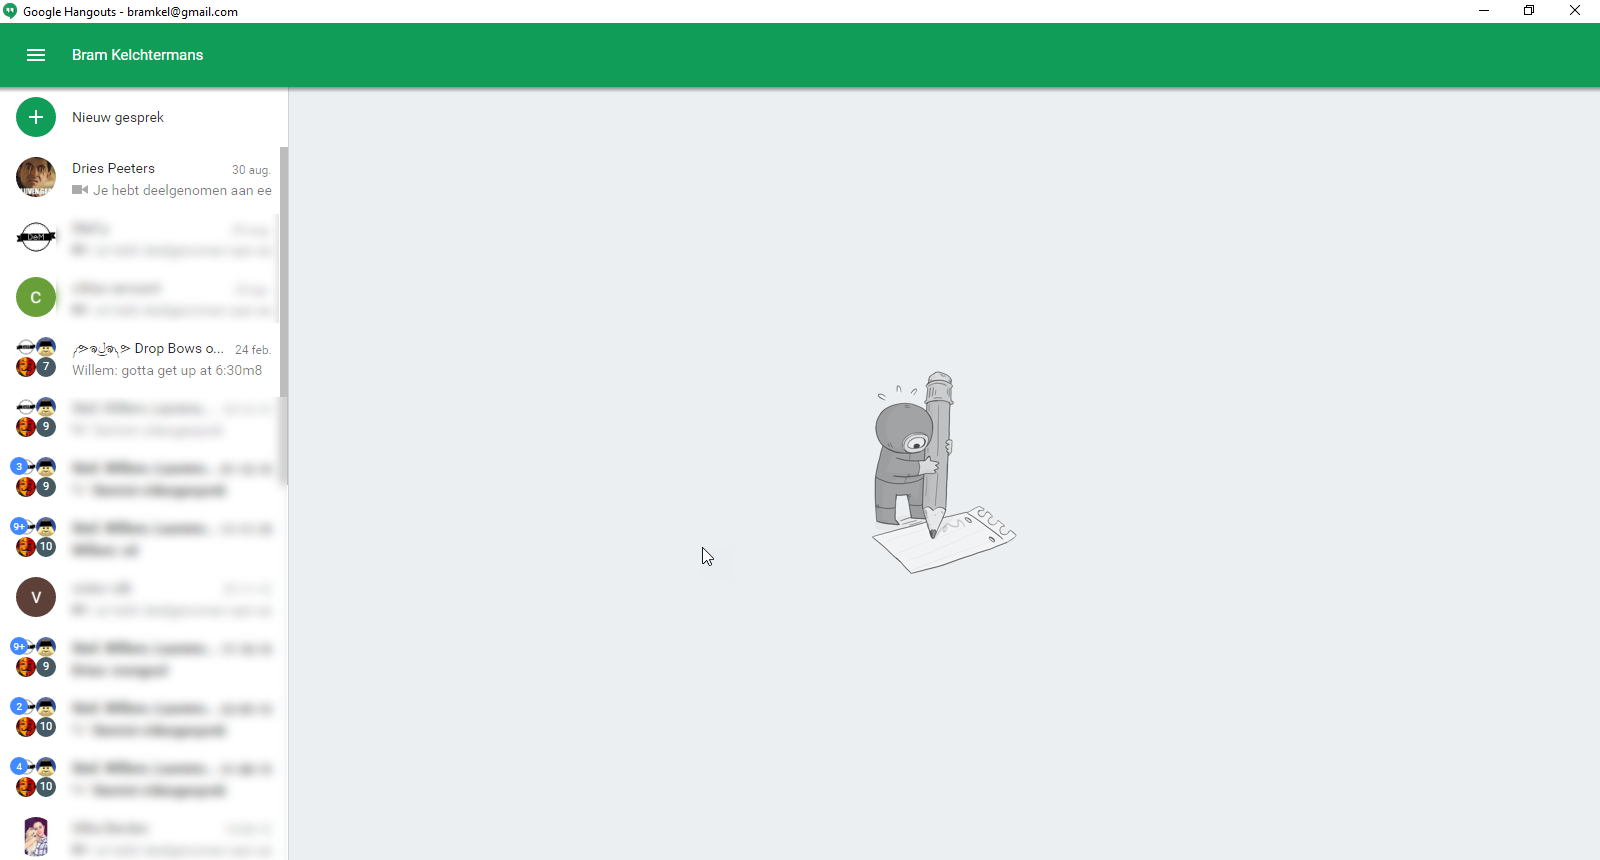
\includegraphics[width=1\textwidth]{Bram_ScreenshotGH1.png}
	\caption{Beginscherm van Hangouts}
	\label{fig:BeginHangouts}
\end{figure}
\begin{figure}
	\centering
	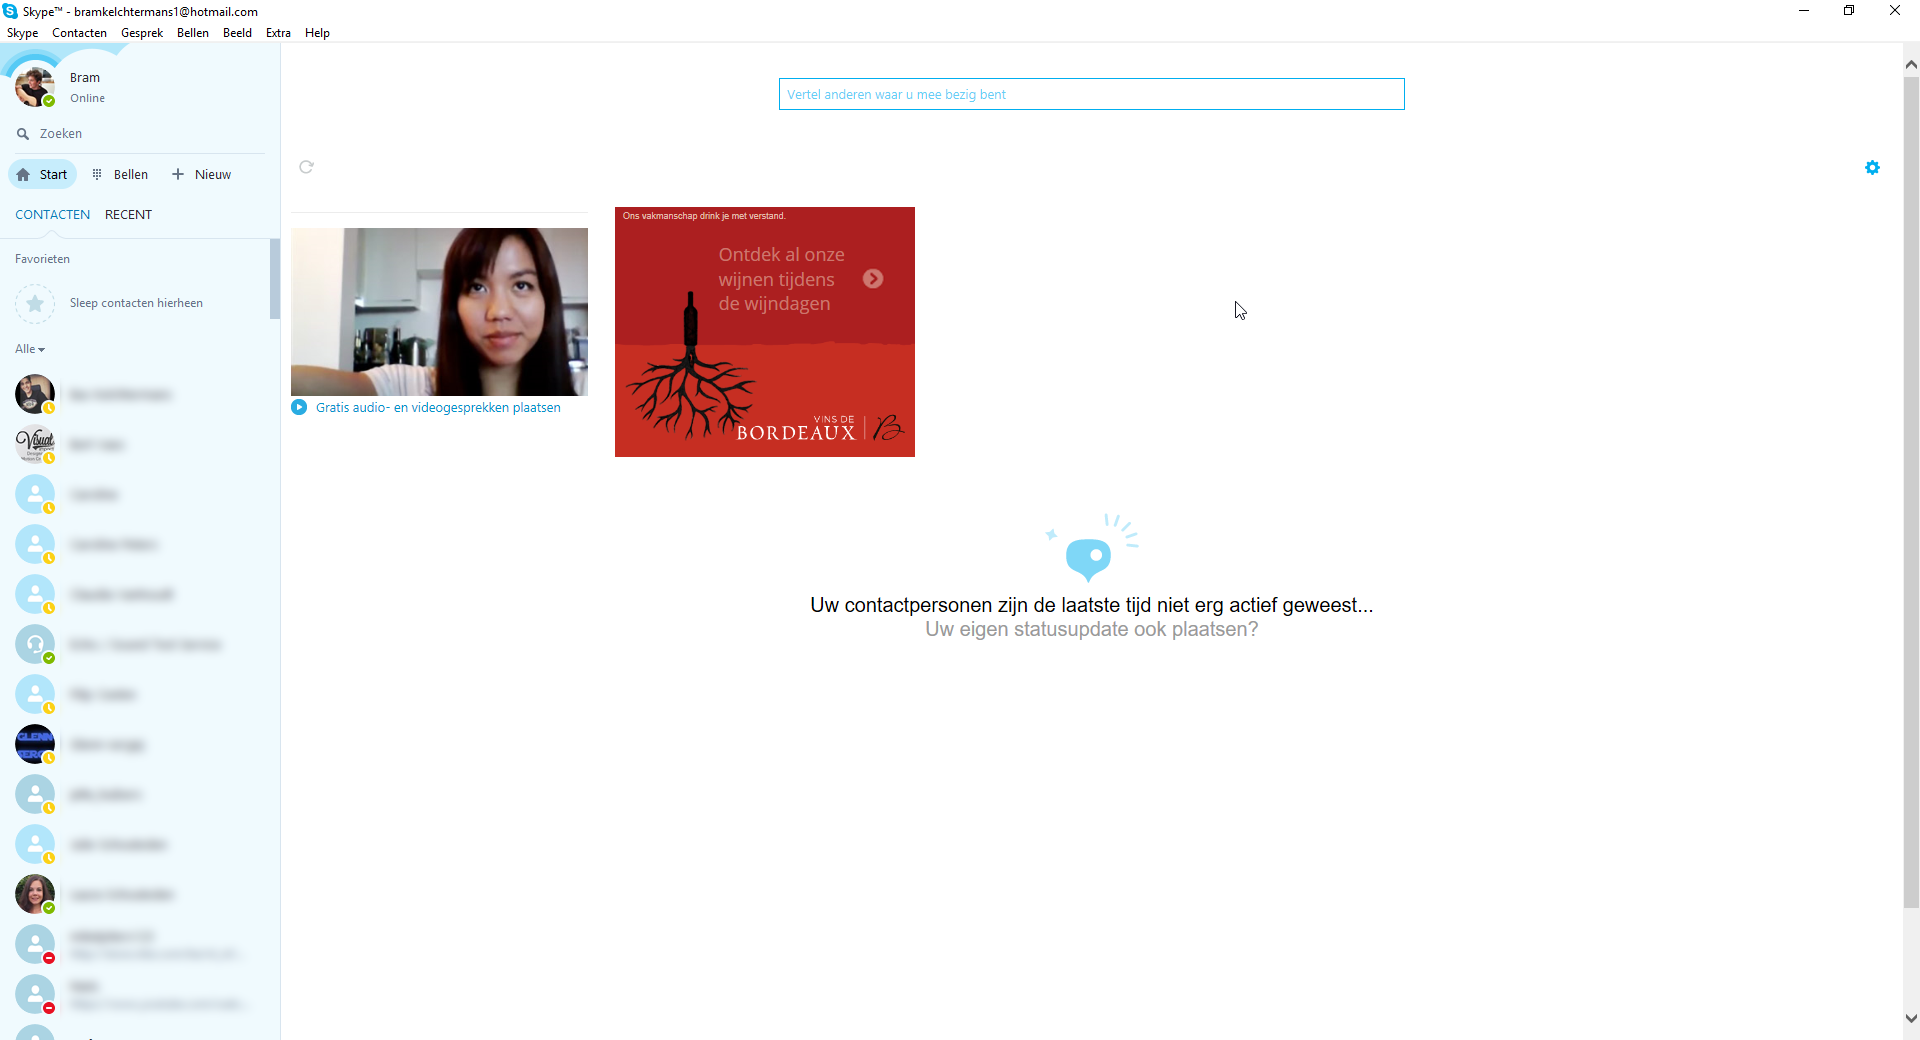
\includegraphics[width=1\textwidth]{Bram_ScreenshotSkype1.png}
	\caption{Beginscherm van Skype}
	\label{fig:BeginSkype}
\end{figure}
\subsubsection{Feedback}
Bij beide applicaties wordt er goed gebruik gemaakt van feedback. Zo wordt er telkens wanneer de gebruiker iemand belt een beltoon gespeeld, dit zodat de gebruiker weet dat de contactpersoon het verzoek om te bellen aan het ontvangen is. De ontvanger van de oproep hoort dan weer een beltoon op zijn of haar computer die aangeeft dat er iemand belt. Wanneer de contactpersoon echter niet bereikbaar is, krijgt de gebruiker duidelijk te horen dat de oproep niet beantwoord werd.
\newline
Een ander voorbeeld van feedback is te zien in figuur \ref{fig:VerzoekHangouts} voor Hangouts en in figuur \ref{fig:VerzoekSkype} voor Skype. In beide gevallen heeft de gebruiker een verzoek gestuurd om contactpersonen te worden met een persoon. Om te bevestigen dat de desbetreffende persoon een verzoek heeft ontvangen gebruiken beide applicaties een tekstboodschap als feedback. In beide applicaties wordt er in de chatsessie veel feedback gegeven. Zo kan men de chatsessie zelf zien, maar ook het startmoment en duur van een spraakgesprek.
\begin{figure}
	\centering
	
\includegraphics[width=0.7\textwidth]{Bram_ScreenshotGH2.png}
	\caption{Contactverzoek in Google Hangouts}
	\label{fig:VerzoekHangouts}
\end{figure}
\begin{figure}
	\centering
	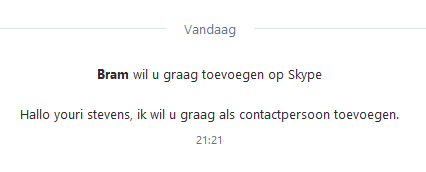
\includegraphics[width=0.7\textwidth]{Bram_ScreenshotSkype2.png}
	\caption{Contactverzoek in Skype}
	\label{fig:VerzoekSkype}
\end{figure}
\newline
Beide applicaties zijn dus voorzien van zowel auditieve als tekstgebaseerde feedback. Dit is dan ook van groot belang in de context van dergelijke applicaties.
\subsection{Metaforen}
\newpage

\section{Bespreking Dylan}
Individuele bespreking (twee tot drie bladzijden, 800 à 1200 woorden)
\subsection{Ontwerpprincipes van Norman}
\subsection{Metaforen}
\newpage


\section{Conclusie}

\newpage
\end{document}